%
% Copyright (c) 2021 Antonio Coín Castro
%
% This work is licensed under a
% Creative Commons Attribution-ShareAlike 4.0 International License.
%
% You should have received a copy of the license along with this
% work. If not, see <http://creativecommons.org/licenses/by-sa/4.0/>.
%

\RequirePackage{fix-cm}
\documentclass[10pt, spanish, professionalfonts]{beamer}

\usepackage{pifont}  % xmark, cmark
\newcommand{\cmark}{\ding{51}}%
\newcommand{\xmark}{\ding{55}}%

% OPCIONES DE BEAMER

\definecolor{Maroon}{cmyk}{0, 0.87, 0.88, 0.1}
\definecolor{teal}{rgb}{0.0, 0.45, 0.45}

\usetheme[block=fill, subsectionpage=progressbar, titleformat section=smallcaps]{metropolis}
\setbeamertemplate{frametitle continuation}[roman]
\setbeamertemplate{section in toc}[balls numbered]
\setbeamertemplate{subsection in toc}[subsections unnumbered]
%\setsansfont[BviejoFont={Fira Sans SemiBold}]{Fira Sans Book}  % Increase font weigth
\widowpenalties 1 10000
\raggedbottom

% COLORES
\setbeamercolor{palette primary}{bg=teal}
\setbeamercolor{progress bar}{use=Maroon, fg=Maroon}

% PAQUETES

\usepackage[utf8]{inputenc}
\usepackage[absolute,overlay]{textpos}
\usepackage[spanish, es-nodecimaldot]{babel}
\usepackage{microtype}
\usepackage{epigraph}
\usepackage{hyperref}
\usepackage{amssymb, amsmath, amsthm, amsfonts, amscd}
\usepackage{listings}

% FONTS
%\usefonttheme{professionalfonts}
%\usepackage{mathpazo}
%\usepackage{eulervm}

\definecolor{backg}{HTML}{F2F2F2} % Fondo
\definecolor{comments}{HTML}{a8a8a8} % Comentarios
\definecolor{keywords}{HTML}{08388c} % Palabras clave
\definecolor{strings}{HTML}{0489B1}  % Strings

\lstset{
language=scala,
basicstyle=\footnotesize\ttfamily,
breaklines=true,
keywordstyle=\color{keywords},
commentstyle=\color{comments},
stringstyle=\color{strings},
xleftmargin=.5cm,
tabsize=2,
% Acentos, ñ, ¿, ¡ (tex.stackexchange.com/questions/24528)
extendedchars=true
}

% COMANDOS PERSONALIZADOS

\let\lmin\wedge
\let\lmax\vee
\newtheorem{prop}{Proposición}
\newtheorem{teorema}{Teorema}
\newtheorem{defi}{Definición}
\newcommand\ddfrac[2]{\frac{\displaystyle #1}{\displaystyle #2}}  % Fracción grande

% TÍTULO

\title{Métodos Bayesianos en modelos RKHS para regresión funcional}
\providecommand{\subtitle}[1]{}
\subtitle{Borrador de ideas y resultados preliminares}
\date{\today \\}
\author{Antonio Coín \\ José R. Berrendero \\ Antonio Cuevas\\}
\institute{Universidad Autónoma de Madrid \\ \textit{Departamento de Matemáticas}}

\titlegraphic{
  \begin{textblock*}{2cm}(9.8cm,6.3cm)
    
\includegraphics[width=2cm]{img/logo-uam}
  \end{textblock*}
}
% DOCUMENTO

\begin{document}
\maketitle

\section{Regresión Lineal Funcional Bayesiana}

\subsection{Marco teórico}

\begin{frame}{Planteamiento Bayesiano}
  \textbf{Modelo RKHS:} \(Y = \alpha_0 + \Psi_{X}^{-1}(\alpha) + \epsilon\), donde \(\alpha\in \mathcal H_K\) y \(\epsilon \sim \mathcal N(0, \sigma^2)\), i.e.:
  \[
    Y_i\mid \theta, X_i=x_i \sim \mathcal N\left(\alpha_0 + \sum_{j=1}^p \beta_jx_i(\tau_j), \ \sigma^2\right).
  \]

\textbf{Distribuciones a priori:}
\begin{align*}
  \pi(\alpha_0, \log \sigma)              & \propto 1,                                                     \\
  \tau                     & \sim \mathcal U([0, 1]^p),                                              \\
  \beta\mid \tau, \sigma^2 & \sim \mathcal N\left(b_0, g\sigma^2\left[\mathcal X_\tau' \mathcal X_\tau + \eta \lambda_{\text{max}}(\mathcal X_\tau' \mathcal X_\tau)\right]^{-1}\right),
\end{align*}

\textbf{Log-posterior:}
\begin{align*}
  \log \pi(\beta, \tau, \alpha_0, \log\sigma\mid \boldsymbol{Y}) &\propto \frac{1}{2}\log |G_\tau| - (p+n)\log \sigma\\
  &-\frac{1}{2\sigma^2} \left(\|\boldsymbol{Y}-\alpha_0\boldsymbol{1} - \mathcal X_\tau\beta\|^2 + \frac{1}{g}(\beta - b_0)'G_\tau(\beta - b_0) \right).
\end{align*}
\end{frame}

\begin{frame}{Modelo Bayesiano}
  \begin{figure}
    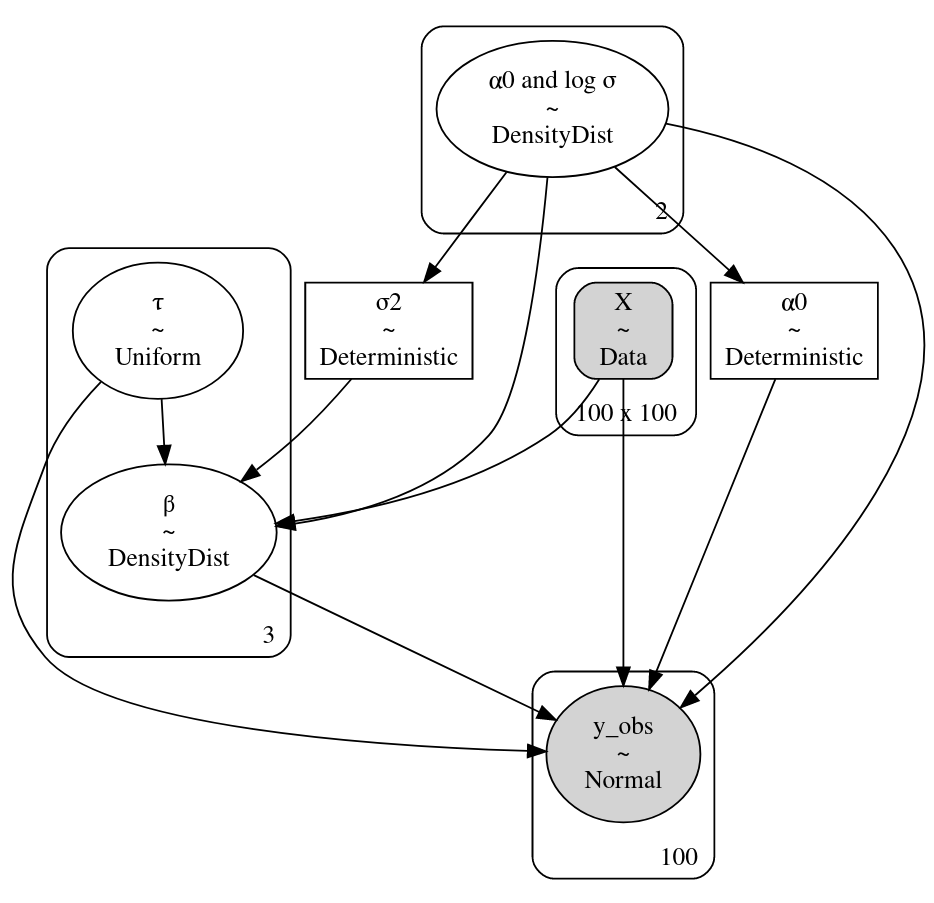
\includegraphics[width=.6\textwidth]{img/modelo_lin}
    \caption{Relaciones entre los parámetros del modelo.}
  \end{figure}
\end{frame}

\begin{frame}{Aproximación de la posteriori}
  \textbf{Procedimiento:} Utilizar métodos MCMC para aproximar la distribución a posteriori. En concreto, se barajan tres alternativas:
  \begin{itemize}
    \item {\color{Maroon}\textit{Affine-Invariant Ensemble Sampler (emcee)}}. Conjunto de cadenas que se influencian mutuamente para dar cada paso.
    \item \textit{NUTS}. Algoritmo que utiliza información del gradiente de la función objetivo para dar cada paso.
    \item \textit{Metropolis}. Algoritmo estándar de \textit{markov chain monte carlo}.
  \end{itemize}

  \vspace{1em}

  Los resultados entre \textit{NUTS} y \textit{emcee} son similares.
\end{frame}

\begin{frame}{Estimación de máxima verosimilitud}
  Una primera aproximación consiste en estimar directamente los parámetros por máxima verosimilitud mediante un enfoque computacional.
  \begin{itemize}
    \item Usamos el algoritmo estocástico \textit{basin-hopping}, un método de dos fases que combina minimización local con un procedimiento de salto global.
    \item Como algoritmo de minimización local escogemos el método quasi-Newton \textit{L-BFGS-B}, que permite especificar restricciones para \(\tau\).
    \item Como el algoritmo implica aleatoriedad, hacemos varias ejecuciones independientes y elegimos la estimación que proporcione un mayor valor del \textit{likelihood}.
  \end{itemize}
\end{frame}

\begin{frame}{Model checking}
  \begin{itemize}
    \item Análisis de la traza de las cadenas y de la distribución a posteriori de los parámetros. Se obtienen \textbf{intervalos creíbles} para los parámetros.
    \item En cada paso obtenemos una estimación \(\tilde \theta_m\), y podemos generar \(Y^{(m)*} \mid \theta_m, X\) siguiendo el modelo asumido.
    \item \textit{Bayesian p-values}: \(p=P(T(Y^*)\leq T(Y)\mid Y)\) para ciertas elecciones de \(T\): mínimo, máximo, mediana, media. Se calcula contando la proporción de muestras generadas que cumplen la desigualdad, y se espera que esté en torno a \(0.5\).
  \end{itemize}

\end{frame}

\begin{frame}{Model checking II}
  \begin{figure}
    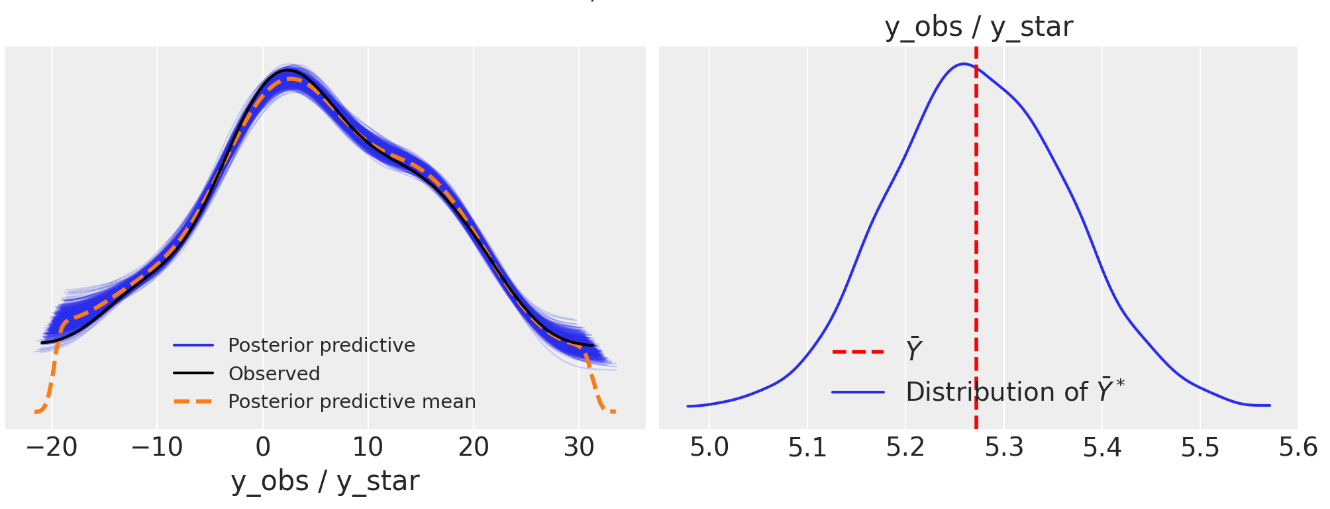
\includegraphics[width=\textwidth]{img/ppc_lin}
    \caption{\textit{Posterior predictive checks} bajo un modelo RKHS.}
  \end{figure}
\end{frame}

\begin{frame}{Predicciones}
  \textbf{Estimación puntual}: Se resume la distribución a posteriori de los parámetros \(\theta\mid Y\) mediante un estimador puntual (media, mediana, moda), y se utilizan para predecir según el modelo:
  \[
  \hat Y_i =\hat \alpha_0 + \sum_{j=1}^p \hat \beta_j x_i(\hat \tau_j), \quad i=1,\dots, n.
  \]

  \textbf{Estimación distribucional}: Se utiliza la media de \textit{todas}  las muestras generadas de \(Y^*\) como predicción:
  \[
    \hat Y = \frac{1}{M}\sum_{m=1}^M Y^{(j)*}.
  \]

  En ambos casos se puede considerar solo una de cada \(k\) muestras.
\end{frame}

\begin{frame}{Predicciones II}
    Podemos hacer también una selección de \(p\) variables usando los estimadores puntuales de \(\tau \mid Y\), y después aplicar cualquier algoritmo de regresión lineal.

    \begin{figure}
      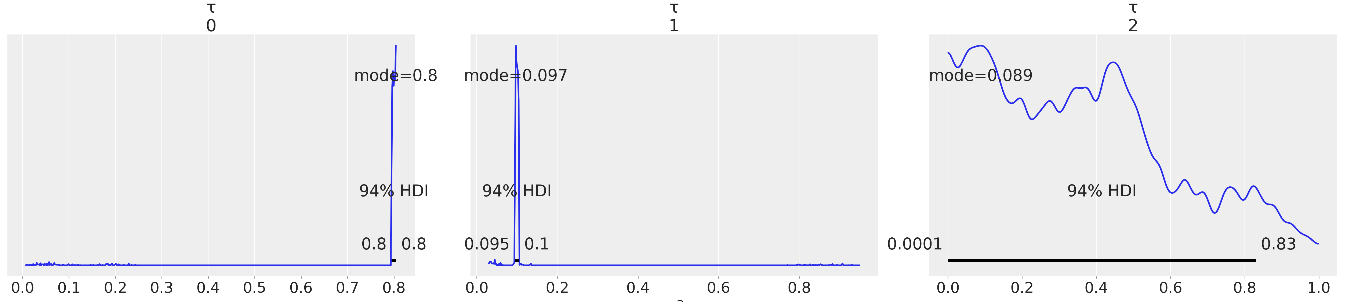
\includegraphics[width=\textwidth]{img/tau_posterior_lin}
      \caption{Distribución a posteriori estimada para los puntos de impacto.}
    \end{figure}

    En cualquier caso, medimos el error usando el MSE como métrica.
\end{frame}

\subsection{Experimentos}

\begin{frame}{Datos sintéticos}
  Se consideran 150 ejemplos de \(X \sim GP(0, K(s, t))\) y tres posibles variantes de \(K\): movimiento browniano fraccional (\(H=0.8\)), Ornstein-Uhlenbeck y kernel RBF.

  Se genera la respuesta \(Y\) acorde a dos modelos, RKHS y \(L^2\). Concretamente, se elige
  \[
    Y_i \sim \mathcal N\big(5 -5X_i(0.1) + 10X_i(0.8), \ 0.5\big)
  \]
  ó
  \[
    Y_i \sim \mathcal N\left(5 + \int_0^1 \log(1+4t)X_i(t)\, dt, \ 0.5\right).
  \]

Consideramos una malla regular de \(N=100\) puntos en \([0, 1]\), y un reparto de 100 ejemplos para entrenamiento y 50 para evaluación.
\end{frame}

\begin{frame}{Datos reales}
  Se consideran dos conjuntos de datos reales.
  \begin{itemize}
    \item \textbf{Tecator:} Contiene 215 ejemplos de mediciones de \textit{absorbancia} en muestras de carne para intentar predecir su contenido en grasa.
    \item \textbf{Aemet}: Contiene 73 ejemplos de curvas de temperatura, a partir de las cuales se intenta predecir la precipitación total.
  \end{itemize}

  En ambos casos hacemos una división \(80\%-20\%\) para entrenamiento y \textit{test}.
\end{frame}

\begin{frame}{Preprocesado de los datos}
  \begin{itemize}
    \item Se centran los regresores para que tengan media \(0\). Opcionalmente, se pueden estandarizar en cada punto de la malla.
    \item Se permite \textbf{sustituir los datos \(\boldsymbol{X_i}\) por su desarrollo en una base} de Fourier, con un número determinado de coeficientes. De esta forma realizamos un suavizado de las curvas.
  \end{itemize}
\end{frame}

\begin{frame}{Algoritmos de comparación}
  \textbf{Regresión lineal multivariante:} Regresión Lineal estándar, Lasso (\(L^1\)), Ridge (\(L^2\)).

  \textbf{Regresión no lineal multivariante}: SVM con kernel RBF.

  \textbf{Regresión lineal funcional}: Modelo \(L^2\), KNN Funcional.

  \textbf{Reducción de dimensión:} PCA Funcional (proyección sobre coeficientes).

  \textbf{Selección de variables:} Aleatoria.

  \vspace{1em}

  Se entrenan todos ellos sobre el conjunto de entrenamiento, haciendo \textit{5-fold cross validation} para escoger los mejores hiperparámetros en cada caso (valor de regularización, número de componentes, ...).
\end{frame}

\begin{frame}{Metodología experimental}
  \begin{itemize}
  \item Para cada conjunto de datos consideramos tres posibles valores de \(p\) y cuatro posibles valores de \(\eta\):
  \begin{itemize}
    \item[--] \(p\in \{2,3,4\}\) para los datos sintéticos y \(p\in \{3, 4, 5\}\) para los datos reales.
      \item[--] \(\eta \in \{0.01, 0.1, 1.0, 10.0\}\).
  \end{itemize}

  \item Para aumentar la estabilidad hacemos 5 repeticiones de cada modelo. Es decir, entrenamos un total de 60 modelos sobre el conjunto de entrenamiento

  \item Con el \textbf{mejor modelo obtenido} se realiza también una selección de variables basada en los valores de \(\tau\) estimados mediante los distintos estimadores puntuales.
\end{itemize}

Además, repetimos este proceso con los datos suavizados en una base de Fourier con 11 elementos (también con los algoritmos de comparación).
\end{frame}

\begin{frame}{Metodología experimental II}
  Fijamos algunos hiperparámetros:
  \begin{itemize}
    \item Número de cadenas: 64.
    \item Número de pasos: 100 + 1000.
    \item Movimientos: elección aleatoria (ponderada) entre dos de los recomendados, \textit{stretch} y \textit{walk}.
    \item Inicialización: Entorno aleatorio del MLE + muestras de las distribuciones a priori.
    \item Prior de \(\beta\): \(b_0\) se elige como el MLE de \(\beta\), y fijamos \(g=5\) (recomendado en \textit{Grollemund et al. (2019)}).
  \end{itemize}
  \vspace{1em}

  \textit{Nota:} El valor de \(g\) no parece afectar al resultado, por lo que podríamos eliminar este parámetro.
\end{frame}

\begin{frame}{Resultados RKHS}
\textbf{Sin base}
  \begin{table}
    \begin{tabular}{c|cc}
      Kernel & Victoria & Victoria sel. variables \\ \hline
      fBM & \cmark & \cmark\\
      O-U & \cmark & \cmark\\
      RBF & \cmark & \cmark
    \end{tabular}
  \end{table}

  \textbf{Base Fourier(11)}
  \begin{table}
    \begin{tabular}{c|cc}
      Kernel & Victoria & Victoria sel. variables \\ \hline
      fBM & \cmark &  \cmark\\
      O-U & \cmark & \xmark\\
      RBF & \cmark & \cmark
    \end{tabular}
  \end{table}
\end{frame}

\begin{frame}{Resultados RKHS II}
  \begin{figure}
    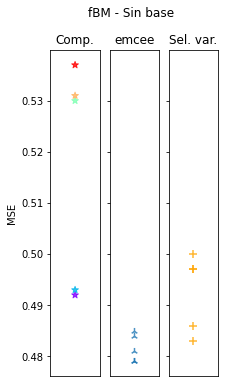
\includegraphics[width=0.3\textwidth]{img/results/lin_rkhs_fbm_nobase}\hfill
    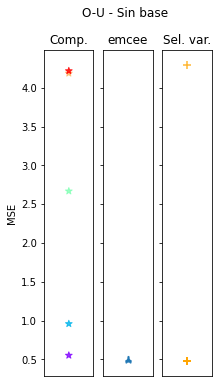
\includegraphics[width=0.3\textwidth]{img/results/lin_rkhs_ou_nobase}\hfill
    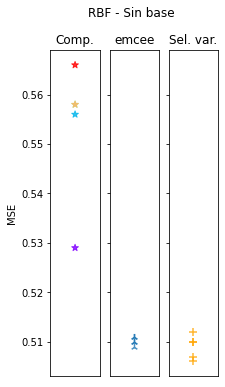
\includegraphics[width=0.3\textwidth]{img/results/lin_rkhs_rbf_nobase}
    \caption{MSE de los 5 mejores modelos en cada caso con el modelo subyacente RKHS y sin usar suavizado con bases. Distinguimos los algoritmos de comparación, nuestro algoritmo Bayesiano (emcee), y nuestra selección de variables Bayesiana.}
  \end{figure}
\end{frame}

\begin{frame}{Resultados RKHS III}
  \begin{figure}
    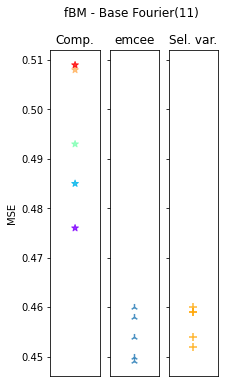
\includegraphics[width=0.3\textwidth]{img/results/lin_rkhs_fbm_base11}\hfill
    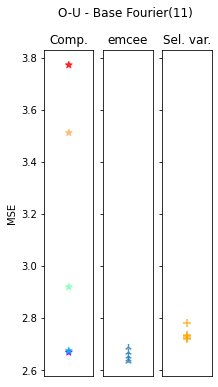
\includegraphics[width=0.3\textwidth]{img/results/lin_rkhs_ou_base11}\hfill
    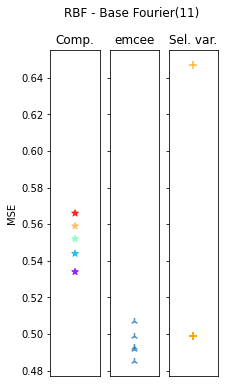
\includegraphics[width=0.3\textwidth]{img/results/lin_rkhs_rbf_base11}
    \caption{MSE de los 5 mejores modelos en cada caso con el modelo subyacente RKHS y con base de Fourier.}
  \end{figure}
\end{frame}

\begin{frame}{Resultados \(\boldsymbol{L^2}\)}
\textbf{Sin base}
  \begin{table}
    \begin{tabular}{c|cc}
      Kernel & Victoria & Victoria sel. variables \\ \hline
      fBM & \xmark & \xmark\\
      O-U & \xmark & \xmark\\
      RBF & \xmark & \xmark
    \end{tabular}
  \end{table}
\textbf{Base Fourier(11)}
  \begin{table}
    \begin{tabular}{c|cc}
      Kernel & Victoria & Victoria sel. variables \\ \hline
      fBM & \cmark &  \cmark\\
      O-U & \cmark & \cmark\\
      RBF & \xmark & \xmark
    \end{tabular}
  \end{table}
\end{frame}

\begin{frame}{Resultados \(\boldsymbol{L^2}\) II}
  \begin{figure}
    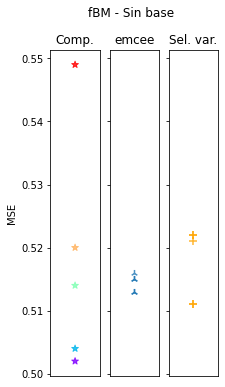
\includegraphics[width=0.3\textwidth]{img/results/lin_l2_fbm_nobase}\hfill
    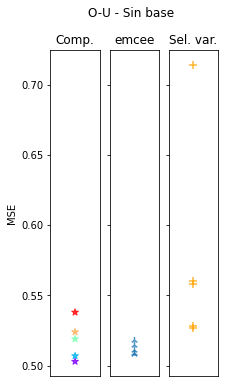
\includegraphics[width=0.3\textwidth]{img/results/lin_l2_ou_nobase}\hfill
    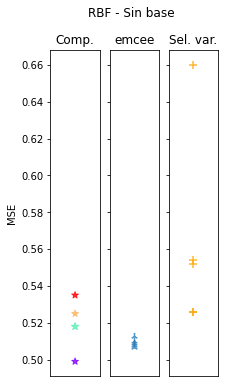
\includegraphics[width=0.3\textwidth]{img/results/lin_l2_rbf_nobase}
    \caption{MSE de los 5 mejores modelos en cada caso con el modelo subyacente \(L^2\) y sin usar suavizado con bases.}
  \end{figure}
\end{frame}

\begin{frame}{Resultados \(\boldsymbol{L^2}\) III}
  \begin{figure}
    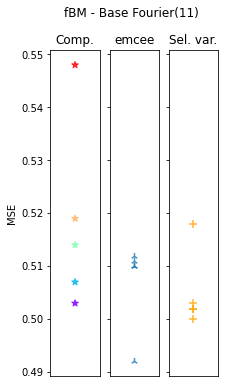
\includegraphics[width=0.3\textwidth]{img/results/lin_l2_fbm_base11}\hfill
    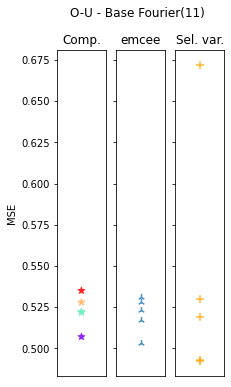
\includegraphics[width=0.3\textwidth]{img/results/lin_l2_ou_base11}\hfill
    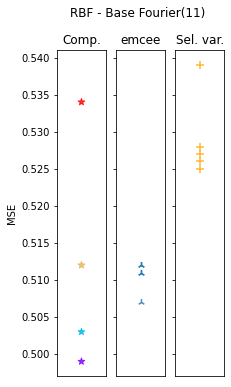
\includegraphics[width=0.3\textwidth]{img/results/lin_l2_rbf_base11}
    \caption{MSE de los 5 mejores modelos en cada caso con el modelo subyacente \(L^2\) y con base de Fourier.}
  \end{figure}
\end{frame}

\begin{frame}{Resultados datos reales}
\textbf{Sin base}
  \begin{table}
    \begin{tabular}{c|cc}
      Dataset & Victoria & Victoria sel. variables \\ \hline
      Tecator & \xmark & \xmark\\
      Aemet & \xmark & \cmark\\
    \end{tabular}
  \end{table}

  \textbf{Base Fourier(11)}
  \begin{table}
    \begin{tabular}{c|cc}
      Dataset & Victoria & Victoria sel. variables \\ \hline
      Tecator & \xmark &  \xmark\\
      Aemet & \xmark & \cmark\\
    \end{tabular}
  \end{table}
\end{frame}

\begin{frame}{Resultados datos reales II}
  \begin{figure}
    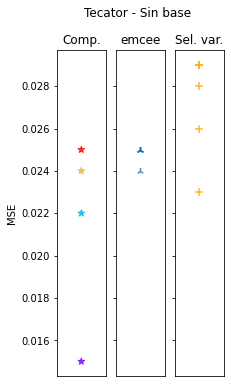
\includegraphics[width=0.3\textwidth]{img/results/lin_tecator_nobase}\hspace{5em}
    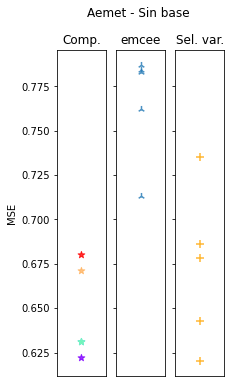
\includegraphics[width=0.3\textwidth]{img/results/lin_aemet_nobase}
    \caption{MSE de los 5 mejores modelos en cada caso con datos reales y sin usar suavizado con bases.}
  \end{figure}
\end{frame}

\begin{frame}{Resultados datos reales III}
  \begin{figure}
    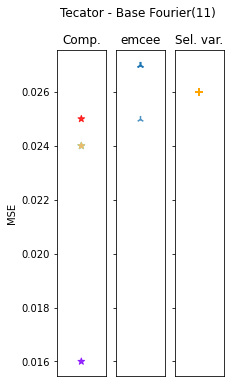
\includegraphics[width=0.3\textwidth]{img/results/lin_tecator_base11}\hspace{5em}
    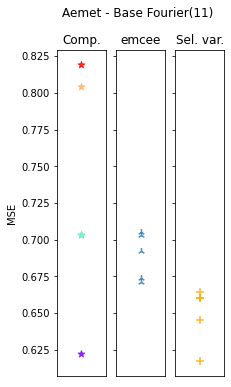
\includegraphics[width=0.3\textwidth]{img/results/lin_aemet_base11}
    \caption{MSE de los 5 mejores modelos en cada caso con datos reales y con base de Fourier.}
  \end{figure}
\end{frame}

\begin{frame}{Algunas observaciones}
\begin{itemize}
  \item Por cada modelo entrenado obtenemos 4 estimadores y 3 estrategias de selección de variables.
  \item En general, se obtienen mejores resultados con el uso de la base.
  \item El tiempo medio de entrenamiento de cada modelo es de unos 20-30 segundos.
  \item En ocasiones, nuestro algoritmo supera con holgura a todos los algoritmos de comparación. Cuando pierde, suele ser frente a uno o dos de ellos (y por poco), pero sigue superando al resto.
  \item Se puede considerar como algoritmo de comparación el estimador de máxima verosimilitud de los parámetros. En casi todas las pruebas experimentales, el desempeño de nuestro algoritmo supera al del MLE.
\end{itemize}


\end{frame}

\begin{frame}{Dificultades}
  \begin{itemize}


  \item Hay multitud de grados de libertad: estandarización de regresores y/o variable respuesta, elección o no de una base (¿cuál?,) algoritmo de estimación del MLE, número, longitud y movimientos de las cadenas MCMC, elección de distribuciones a priori, elección de \(g, b_0\) y \(\eta\), etc.
  \item El algoritmo MCMC es costoso, y en conjuntos de datos grandes las estrategias de \textit{cross-validation} para seleccionar parámetros pueden no ser viables.
  \item Es necesario un procedimiento para seleccionar el valor de \(p\) (BIC, WAIC, WBIC, \textit{cross-validation}, ...).
  \item Debido a la aleatoriedad del algoritmo, los resultados pueden variar sustancialmente de una ejecución a otra.
  \item La distribución a priori para \(\beta\) depende en gran medida del valor de \(b_0\) escogido. Si su estimación inicial no es buena, el algoritmo no funciona demasiado bien.
\end{itemize}
\end{frame}

\begin{frame}{Dificultades II}
  \begin{itemize}
    \item Hay un problema de \textit{identificabilidad} de los coeficientes (son intercambiables), que se agudiza especialmente al usar varias cadenas.
    \item En el caso en el que el modelo subyacente es RKHS, es posible que no se recuperen los verdaderos valores de los parámetros debido a interacciones entre los coeficientes (si \(p\) es mayor que el número real de componentes).
    \item El uso de distribuciones a priori impropias implica comprobar que \(\int_{\Theta} \pi(Y\mid \theta)\pi(\theta)\, d\theta < \infty\).
  \end{itemize}
\end{frame}

\begin{frame}{Alternativas}
  \begin{itemize}
    \item Explorar el concepto de \textit{online learning} aplicado a esta situación, por ejemplo usando como priori de nuevos datos la posteriori aprendida. Estudiar la \textbf{consistencia} de la distribución a posteriori.
    \item Utilizar otras herramientas de suavizado en lugar de bases de Fourier.
    \item Sustitutir la distribución a priori de \(\beta\) por otra que requiera menos hiperparámetros.
    \item Sustituir las distribuciones impropias por otras propias.
  \end{itemize}

\end{frame}

\section{Regresión Logística Funcional Bayesiana}

\subsection{Marco teórico}

\begin{frame}{Planteamiento Bayesiano}
\textbf{Modelo}: Cada \(Y_i\) se puede ver como una variable aleatoria de Bernoulli \(\mathcal B(p(x_i))\), con
\[
p_i \equiv p(x_i)=\mathbb P(Y_i=1\mid X_i=x_i) = \frac{1}{1 + \exp\left\{-\alpha_0-\displaystyle\sum_{j=1}^p \beta_jx_i(\tau_j)\right\}}.
\]

\textbf{Distribuciones a priori}: Igual que en regresión lineal.

\textbf{Log-posterior}:
\begin{align*}
  \log \ &\pi(\beta, \tau, \alpha_0, \log\sigma\mid Y) \propto\\
   &\sum_{i=1}^n \left[ \left(\alpha_0 + \Psi^{-1}_{x_i}(\alpha)\right)y_i - \log\left(1 + \exp\left\{\alpha_0 + \Psi_{x_i}^{-1}(\alpha)\right\}\right)\right]\\
   &+
\frac{1}{2}\log |G_\tau| - p\log \sigma -\frac{1}{2g\sigma^2} (\beta - b_0)'G_\tau(\beta - b_0).
\end{align*}
\end{frame}

\begin{frame}{Model checking}
  \begin{figure}
    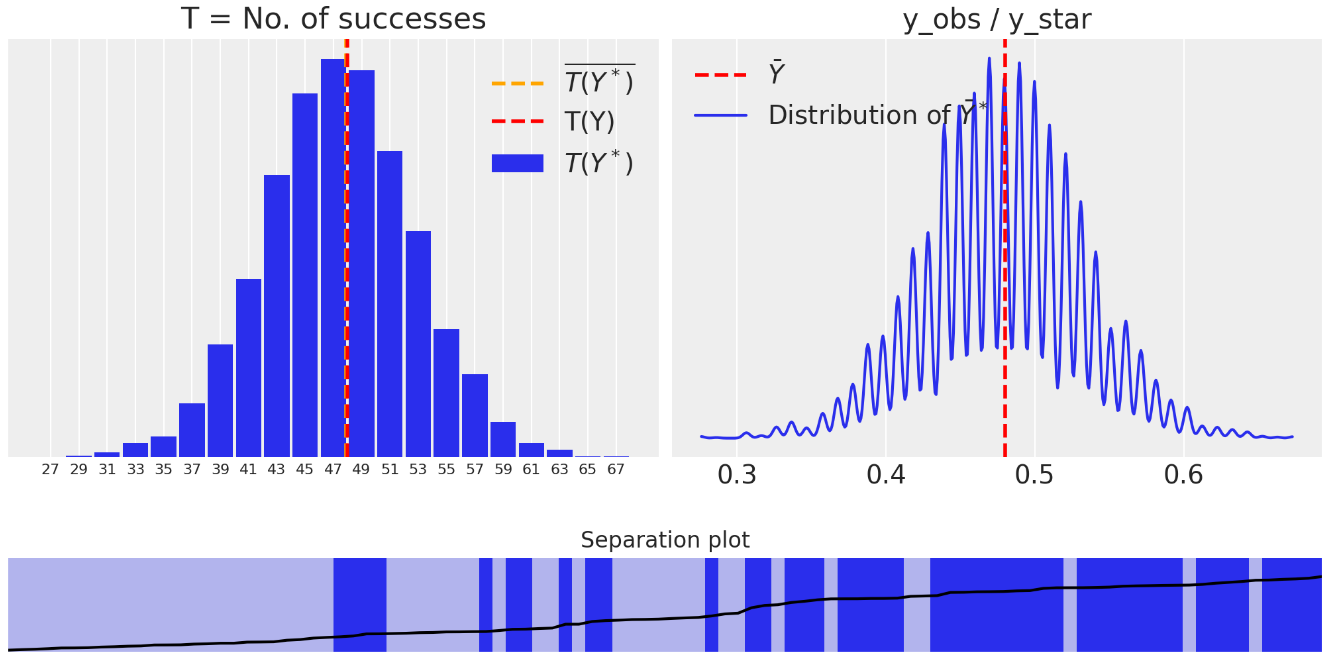
\includegraphics[width=\textwidth]{img/ppc_log}
    \caption{\textit{Posterior predictive checks} bajo un modelo RKHS.}
  \end{figure}
\end{frame}

\begin{frame}{Predicciones}

\begin{itemize}
  \item Fijamos un umbral en \(0.5\) para establecer la pertenencia a las clases.
   \item Los estimadores puntuales y la selección de variables son análogos al caso de regresión lineal.
   \item Tenemos ahora dos estimadores basados en la distribución a posteriori (similares a los \textit{ensembles} de clasificadores):
   \begin{itemize}
     \item[--] Basado en el voto mayoritario de las muestras \(Y^*\) generadas.
     \item[--] Basado en la media de las probabilidades \(p_i^*\) generadas (con aplicación posterior del umbral).
   \end{itemize}
  \item Se usa el \textit{accuracy} (precisión) para evaluar los modelos.
\end{itemize}
\end{frame}

\subsection{Experimentos}

\begin{frame}{Datos sintéticos}
Seguimos la misma estrategia de generación de datos antes. Se consideran las mismas tres funciones de covarianza y se genera la respuesta tanto con un modelo RKHS como L2, i.e.:
  \[
    Y_i \sim \mathcal B\left(\frac{1}{1 + \exp\left\{0.5 + 5X_i(0.1) - 10X_i(0.8)\right\}}\right)
  \]
  ó
  \[
    Y_i \sim \mathcal B\left(\frac{1}{1 + \exp\left\{0.5 -\int_0^1 \log(1+4t)X_i(t)\, dt\right\}}\right).
  \]

  \vspace{1em}

  Se introduce un pequeño ruido aleatorio en las etiquetas, y además se intenta que ambas clases estén balanceadas.

\end{frame}

\begin{frame}{Datos reales}
  Se consideran dos conjuntos de datos reales.
  \begin{itemize}
    \item \textbf{Medflies:} Contiene 534 ejemplos de mediciones del número de huevos diario puesto por una serie de moscas, para intentar predecir si viven mucho o poco.
    \item \textbf{Growth}: Contiene 93 ejemplos de curvas de altura en niños y niñas.
  \end{itemize}

  En ambos casos hacemos una división \(80\%-20\%\) para entrenamiento y \textit{test}.
\end{frame}

\begin{frame}{Algoritmos de comparación}
  \textbf{Clasificación lineal multivariante:} Regresión Logística, SVM lineal.

  \textbf{Clasificación no lineal multivariante}: SVM con kernel RBF.

  \textbf{Clasificación funcional}: \textit{Maximum Depth}, \textit{Nearest Centroid} Funcional, KNN Funcional.

  \textbf{Reducción de dimensión:} PCA Funcional (proyección sobre coeficientes).

  \textbf{Selección de variables:} Aleatoria, \textit{Recursive Maxima Hunting}, \textit{RKVS} (Mahalanobis).

  \vspace{1em}

  Mismo preprocesado y metodología experimental que en el caso de regresión lineal, utilizando esta vez 9 coeficientes de Fourier.
\end{frame}

\begin{frame}{Resultados RKHS}
\textbf{Sin base}
  \begin{table}
    \begin{tabular}{c|cc}
      Kernel & Victoria & Victoria sel. variables \\ \hline
      fBM & \xmark & \xmark\\
      O-U & \xmark & \cmark\\
      RBF & \cmark & \xmark
    \end{tabular}
  \end{table}

  \textbf{Base Fourier(9)}
  \begin{table}
    \begin{tabular}{c|cc}
      Kernel & Victoria & Victoria sel. variables \\ \hline
      fBM & \cmark &  \cmark\\
      O-U & \cmark & \cmark\\
      RBF & \cmark & \cmark
    \end{tabular}
  \end{table}
\end{frame}

\begin{frame}{Resultados RKHS II}
  \begin{figure}
    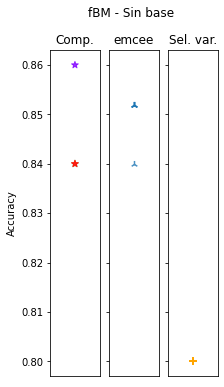
\includegraphics[width=0.3\textwidth]{img/results/log_rkhs_fbm_nobase}\hfill
    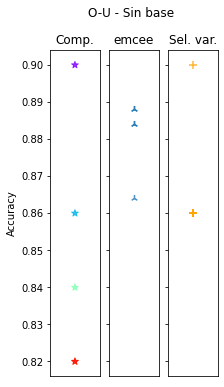
\includegraphics[width=0.3\textwidth]{img/results/log_rkhs_ou_nobase}\hfill
    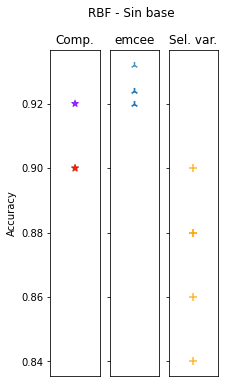
\includegraphics[width=0.3\textwidth]{img/results/log_rkhs_rbf_nobase}
    \caption{Precisión de los 5 mejores modelos en cada caso con el modelo subyacente RKHS y sin usar suavizado con bases. Distinguimos los algoritmos de comparación, nuestro algoritmo Bayesiano (emcee), y nuestra selección de variables Bayesiana.}
  \end{figure}
\end{frame}

\begin{frame}{Resultados RKHS III}
  \begin{figure}
    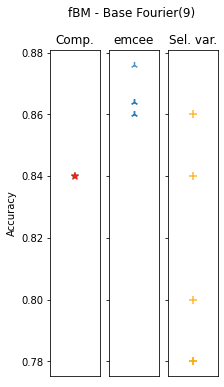
\includegraphics[width=0.3\textwidth]{img/results/log_rkhs_fbm_base9}\hfill
    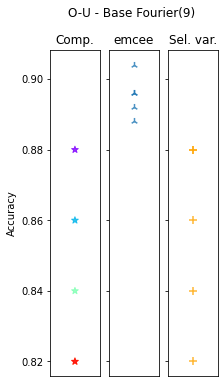
\includegraphics[width=0.3\textwidth]{img/results/log_rkhs_ou_base9}\hfill
    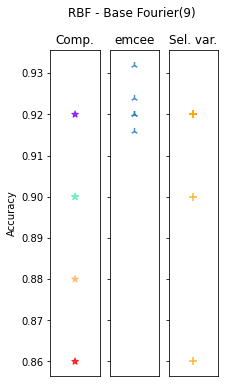
\includegraphics[width=0.3\textwidth]{img/results/log_rkhs_rbf_base9}
    \caption{Precisión de los 5 mejores modelos en cada caso con el modelo subyacente RKHS y con base de Fourier.}
  \end{figure}
\end{frame}

\begin{frame}{Resultados \(\boldsymbol{L^2}\)}
\textbf{Sin base}
  \begin{table}
    \begin{tabular}{c|cc}
      Kernel & Victoria & Victoria sel. variables \\ \hline
      fBM & \xmark & \xmark\\
      O-U & \cmark & \xmark\\
      RBF & \cmark & \cmark
    \end{tabular}
  \end{table}

  \textbf{Base Fourier(9)}
  \begin{table}
    \begin{tabular}{c|cc}
      Kernel & Victoria & Victoria sel. variables \\ \hline
      fBM & \xmark &  \cmark\\
      O-U & \xmark & \cmark\\
      RBF & \cmark & \cmark
    \end{tabular}
  \end{table}
\end{frame}

\begin{frame}{Resultados \(L^2\) II}
  \begin{figure}
    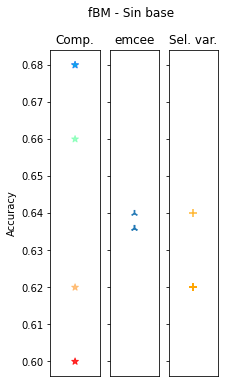
\includegraphics[width=0.3\textwidth]{img/results/log_l2_fbm_nobase}\hfill
    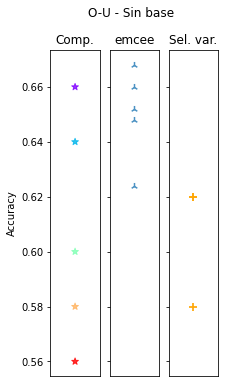
\includegraphics[width=0.3\textwidth]{img/results/log_l2_ou_nobase}\hfill
    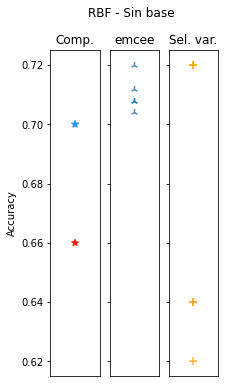
\includegraphics[width=0.3\textwidth]{img/results/log_l2_rbf_nobase}
    \caption{Precisión de los 5 mejores modelos en cada caso con el modelo subyacente \(L^2\) y sin usar suavizado con bases.}
  \end{figure}
\end{frame}

\begin{frame}{Resultados \(L^2\) III}
  \begin{figure}
    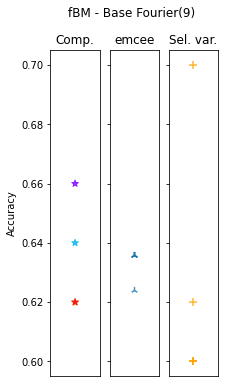
\includegraphics[width=0.3\textwidth]{img/results/log_l2_fbm_base9}\hfill
    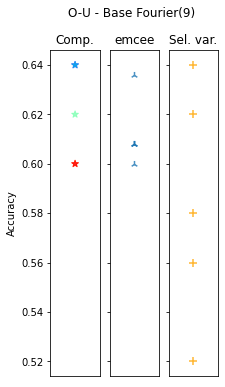
\includegraphics[width=0.3\textwidth]{img/results/log_l2_ou_base9}\hfill
    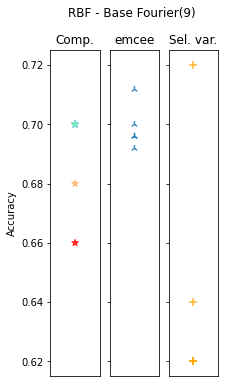
\includegraphics[width=0.3\textwidth]{img/results/log_l2_rbf_base9}
    \caption{Precisión de los 5 mejores modelos en cada caso con el modelo subyacente \(L^2\) y con base de Fourier.}
  \end{figure}
\end{frame}

\begin{frame}{Resultados datos reales}
\textbf{Sin base}
  \begin{table}
    \begin{tabular}{c|cc}
      Dataset & Victoria & Victoria sel. variables \\ \hline
      Medflies & \xmark & \xmark\\
      Growth & \cmark & \cmark\\
    \end{tabular}
  \end{table}

  \textbf{Base Fourier(9)}
  \begin{table}
    \begin{tabular}{c|cc}
      Dataset & Victoria & Victoria sel. variables \\ \hline
      Medflies & \xmark &  \xmark\\
      Growth & \cmark & \cmark\\
    \end{tabular}
  \end{table}

  Tanto en las victorias como en las derrotas, la precisión es muy similar. Podemos considerar un empate en ambos conjuntos.
\end{frame}

\begin{frame}{Resultados datos reales II}
  \begin{figure}
    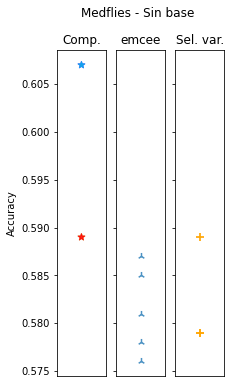
\includegraphics[width=0.3\textwidth]{img/results/log_medflies_nobase}\hspace{5em}
    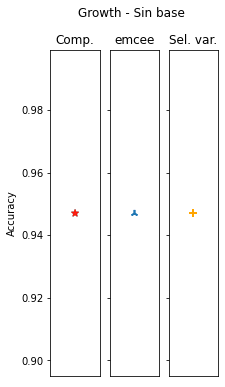
\includegraphics[width=0.3\textwidth]{img/results/log_growth_nobase}
    \caption{Precisión de los 5 mejores modelos en cada caso con datos reales y sin usar suavizado con bases.}
  \end{figure}
\end{frame}

\begin{frame}{Resultados datos reales III}
  \begin{figure}
    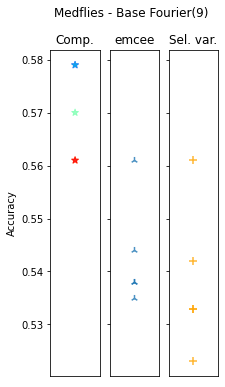
\includegraphics[width=0.3\textwidth]{img/results/log_medflies_base9}\hspace{5em}
    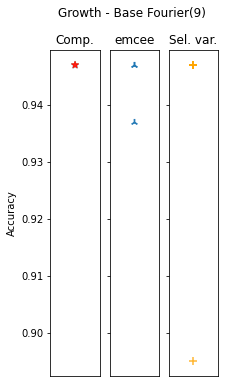
\includegraphics[width=0.3\textwidth]{img/results/log_growth_base9}
    \caption{Precisión de los 5 mejores modelos en cada caso con datos reales y con base de Fourier.}
  \end{figure}
\end{frame}

\end{document}
